\documentclass[12pt,a4paper,openright]{report} %twoside
%-----------------------------------------------------------------
% LaTeX template for a Bachelor Thesis Book (CSE 400) 
% of the Department of Computer Science and Engineering  at the 
% Green University of Bangladesh (GUB)

% Written By: Muhammad Abul Hasan, PhD ( Main Author )

% Date Updated : January 01, 2024 (v1.0) Muhammad Abul Hasan, PhD
% Date Updated : October 17, 2025 (v1.1) Md. Dulal Hossain, Teaching Assistant of Green University of Bangladesh

% For any comments or suggestions: muhammad.hasan@cse.green.edu.bd
%-----------------------------------------------------------
\usepackage{gubcse400}



% ===================== All Necessary Packages =====================

\usepackage{algorithm}          % For creating algorithm environments
\usepackage{listings}           % For including code blocks with syntax highlighting
\usepackage{graphicx}           % For inserting and managing images
\usepackage{booktabs}           % For professional-looking tables
\usepackage{xcolor}             % For colored text and code highlighting
\usepackage{algpseudocode}      % For writing pseudocode within algorithm environment
\usepackage{amsmath}            % For advanced mathematical symbols and environments
\definecolor{codegreen}{rgb}{0,0.6,0} % Define custom color for code elements
\usepackage[a4paper, left=2.5cm, right=2cm, top=2.5cm, bottom=2cm]{geometry} % Page layout settings

\usepackage{rotating}           % For rotating figures, tables, or text
\usepackage[utf8]{inputenc}     % For UTF-8 character encoding support
\usepackage{pifont}             % For special symbols (e.g., checkmarks, crosses)
\usepackage{array}              % For extended table features
\usepackage{cases}              % For the 'cases' environment in math equations
\usepackage{float}              % To control figure/table placement precisely
\usepackage{longtable}          % For multipage tables
\usepackage{makecell}           % For customized cell formatting in tables
\geometry{margin=1in}           % Adjust page margins (alternative geometry setting)
\renewcommand{\arraystretch}{1.3} % Increases row spacing in tables for better readability


% Change the name and designation of Chairperson of dept. as required
\def\HodName{Name of the Chairperson\xspace}
\def\HodPosition{Designation and Position\xspace}
%
%-----------------------------------------------------------
% Set your report/thesis particulars 
%-----------------------------------------------------------
%
% Use one: Thesis/Project report
\def\RoportType{Thesis\xspace} 
%\def\RoportType{Project report\xspace}
%
%
\def\ReportTitle{Title of Thesis\xspace}
\def\Supervisor{Supervisor Name\xspace} 
\def\SupervisorPosition{Supervisor Position\xspace}
\def\secondSupervisor{Co-supervisor Name\xspace} 
\def\secondSupervisorPosition{Co-supervisor Position\xspace}
%
%
%\def\reportSubmissionDate{\today}
\def\reportSubmissionDate{February 01, 2029}
\def\reportSubmissionTerm{Fall 2025}


%-----------------------------------------------------------
% Set your group members' particulars 
%-----------------------------------------------------------
%
\def\numberOfAuthors{1} % write 1, 2 or 3 (depends on group)
%
\def\firstAuthor{First Author\xspace} 
\def\firstAuthorID{243014001\xspace}
\def\firstAuthorDedication{ Dedicated to Almighty Allah —
\\ \textit{All praise to Him for His endless mercy and guidance.\\
Dedicated to my beloved parents for their love and support, and to all who inspired and encouraged me along the way.}}
%
\def\secondAuthor{Second Author\xspace} 
\def\secondAuthorID{243014002\xspace} 
\def\secondAuthorDedication{To my ever-loving and supportive parents,
\\ \textit{whose sacrifices, prayers, and unconditional love
have been my greatest strength.}}
%
\def\thirdAuthor{Third Author\xspace} 
\def\thirdAuthorID{243014003\xspace} 
\def\thirdAuthorDedication{To my respected teachers, mentors, and well-wishers,
\\ \textit{whose knowledge and encouragement
have shaped my academic journey.}}
%
%-----------------------------------------------------------
% Set Board members' particulars 
%-----------------------------------------------------------
%
\def\BoardNumber{10} % board number in which you are going to present your work
%
\def\BoardChair{Board Chair's Name\xspace} 
\def\BoardChairPosition{Board Chair's Position\xspace}
%
\def\BoardMember{Board Member's Name\xspace} 
\def\BoardMemberPosition{Board Member's Position\xspace} 
%
\def\BoardExternalMember{External Member's Name\xspace} 
\def\BoardExternalMemberPosition{External Member's Position\xspace} 
\def\BoardExternalMemberAffiliation{External Member's Affiliation\xspace}
%
%-----------------------------------------------------------
\begin{document}
\input{./Setup/front}
%-----------------------------------------------------------
% Include Chapters 
%-----------------------------------------------------------
 \chapter{Introduction}
\label{introduction}


%\section{Introduction}

%{\color{red} \textbf{  Instruction:} “Introduce the topic of the research and set the foundation for the rest of the work. Begin with a general overview of the subject area, and explain what is being studied and why it matters. Highlight the importance of the chosen field, showing its relevance in academic, industrial, or social contexts.”}

 %\textbf{\color{blue} Example:} Heart disease is one of the \textbf{leading causes of death worldwide}, responsible for \textbf{millions of fatalities} each year. \textbf{Early detection} and \textbf{diagnosis} can significantly reduce \textbf{mortality} by enabling \textbf{timely treatment}. Traditional methods depend heavily on \textbf{manual diagnosis by doctors}, which can be \textbf{time-consuming} and prone to \textbf{human error}. In recent years, \textbf{machine learning (ML)} has emerged as a \textbf{powerful tool} for developing \textbf{automated} and \textbf{accurate prediction systems }[1]. This thesis focuses on building an \textbf{ML-based model} to predict the \textbf{likelihood of heart disease} using \textbf{medical data} such as \textbf{age, blood pressure, cholesterol level}, and other \textbf{clinical factors}. 



\section{Background of the Study} 

{\color{red} \textbf{  Instruction:}  “Give a brief description of how the topic or technology started and how it has evolved over time. Highlight key milestones that shaped its development. Mention important inventions that played a significant role. Discuss major breakthroughs that contributed to its growth and current relevance.”}

 \textbf{\color{blue} Example:} Heart disease research and diagnostic methods \textbf{started} many decades ago and have \textbf{evolved over time} through continuous scientific advancements. Several \textbf{key milestones} shaped its development, including the introduction of \textbf{electrocardiograms (ECG)} and \textbf{cholesterol testing}[2]. Important \textbf{inventions} such as \textbf{advanced imaging techniques} and \textbf{biomarker detection methods} played a significant role in improving diagnosis. Major \textbf{breakthroughs}, including the use of \textbf{machine learning (ML)} for \textbf{predictive modeling}, have contributed to the field’s \textbf{growth} and its \textbf{current relevance} in healthcare[3][4].



\subsection{State of the Art in the Modern Context} 

{\color{red} \textbf{  Instruction:} “Describe the \textbf{current status of the field}, focusing on how it is being used and developed today. Highlight \textbf{recent research contributions, emerging tools}, and \textbf{advanced technologies} that are shaping progress in this area. Discuss the \textbf{current challenges}, such as \textbf{technical limitations, ethical concerns}, or \textbf{practical implementation issues}. Cite a few \textbf{up-to-date research papers or articles} to provide insights into the latest \textbf{developments} and \textbf{trends}.”}

 \textbf{\color{blue} Example:} Today, \textbf{machine learning (ML) models} trained on \textbf{large datasets} can predict \textbf{heart disease risk} with impressive \textbf{accuracy}. Research shows that \textbf{algorithms} such as Random Forest, Support Vector Machines (SVM), and \textbf{deep neural networks} outperform traditional \textbf{scoring systems} like the \textbf{Framingham Risk Score}[5]. Recent studies also incorporate \textbf{hybrid techniques}, such as combining \textbf{feature selection} with \textbf{ensemble learning} to improve \textbf{prediction performance}. Additionally, \textbf{deep learning models} using \textbf{patient ECG signals} and \textbf{wearable sensor data} are being explored in \textbf{current research}, demonstrating ongoing \textbf{innovation} in the field[6].



\subsection{Importance and Relevance of the Topic}

{\color{red} \textbf{  Instruction:} 
“Explain the \textbf{importance of this topic} by emphasizing its \textbf{relevance} and \textbf{impact}. Highlight its \textbf{usefulness} in society, \textbf{industry}, or \textbf{research}, showing how it contributes to \textbf{progress} and \textbf{innovation}. Discuss the \textbf{benefits} that could be achieved by solving this problem, particularly how \textbf{individuals}, \textbf{communities}, or \textbf{organizations} may gain from its solutions.”}


 \textbf{\color{blue} Example:} A heart disease prediction system based on machine learning could be integrated into various healthcare settings to maximize its impact[9]. For example, in rural clinics, it can assist non-specialist doctors by providing quick and reliable risk assessment for both compensating for the shortage of trained cardiologists. In addition, the system can be embedded into mobile health applications through multiple systems, such as healthcare providers, and cardiovascular health conveniently from home. Within hospital usage patterns, such a tool can help prioritize high-cash patients, ensuring that those in urgent need of care receive immediate attention. Beyond these use cases, the system can also reduce the overall diagnostic workload for healthcare professionals, streamline decision-making, and ultimately improve patient outcomes by enabling timely interventions.




%\section{Problem Statement} 
\section{Research Problem and Its Context} 

{\color{red} \textbf{  Instruction:} “Clearly explain the main problem that your work is attempting to solve. Mention any gaps in current systems or existing limitations, and highlight the areas where improvements or solutions are needed.”}

 \textbf{\color{blue} Example:}
 While ML-based heart disease prediction models have shown promising results, many suffer from issues such as overfitting, poor generalization to new data, or reliance on large datasets that are not always available.

This thesis aims to design a model that maintains high prediction accuracy even with small to moderately sized datasets and simple features, while being computationally efficient enough to deploy in low-resource settings [8].


\section{Motivation}

{\color{red} \textbf{  Instruction:} Why this problem is important and worth investigating. Explain the reason the topic was chosen. Mention any personal interest or factors that caused this problem to attract attention.}

 \textbf{\color{blue} Example:} The motivation for pursuing a thesis on heart disease prediction includes:

\begin{itemize}
    \item \textbf{Healthcare Impact:} Contributing to early detection of heart disease to reduce mortality and improve patient outcomes.
    \item \textbf{Technological Advancement:} Applying machine learning techniques to solve real-world healthcare problems.
    \item \textbf{Resource Optimization:} Creating a system that is efficient and usable even in low-resource or rural settings.
    \item \textbf{Research Contribution:} Advancing knowledge in medical AI and providing a foundation for future studies.
    \item \textbf{Practical Application:} Preparing a deployable system that can assist healthcare professionals and patients in decision-making.
    \item \textbf{Data-Driven Insight:} Leveraging clinical and demographic data to develop predictive models for accurate diagnosis.
\end{itemize}

\section{Applications and Practical Use Cases}

{\color{red} \textbf{  Instruction:} Real-world or academic use cases of your research. "Describe the potential real-life applications of the research. Highlight its use in areas such as industry, healthcare, education, or other relevant fields."}

 \textbf{\color{blue} Example:} A heart disease prediction system based on machine learning could be integrated into various healthcare settings to maximize its impact[9]. For example, in rural clinics, it can assist non-specialist doctors by providing quick and reliable risk assessment for both compensating for the shortage of trained cardiologists. In addition, the system can be embedded into mobile health applications through multiple systems, such as healthcare providers, and cardiovascular health conveniently from home. Within hospital usage patterns, such a tool can help prioritize high-cash patients, ensuring that those in urgent need of care receive immediate attention. Beyond these use cases, the system can also reduce the overall diagnostic workload for healthcare professionals, streamline decision-making, and ultimately improve patient outcomes by enabling timely interventions.

\section{Research Objectives }
{\color{red} \textbf{  Instruction:} Clearly define the primary aim and sub-goals of your study. "To interpret the aims of the research. Write one general objective and two to three specific objectives to outline the intended outcomes and focus areas of the study."}

 \textbf{\color{blue} Example:} 
 
 \textbf{General Objective:}
To develop an accurate and reliable machine learning model for predicting heart disease.

\textbf{Specific Objectives:}
To collect and preprocess clinical and demographic data relevant to heart disease.

To identify and select the most important features that influence heart disease prediction.

To design, train, and evaluate different machine learning models to determine the most effective approach.

\section{Research Methodology (Overview) }
{\color{red} \textbf{  Instruction:} "A brief overview of the research methods or approaches used." You can add a conceptual diagram.}

 \textbf{\color{blue} Example:} A simple attack Classification is presented in Fig: \ref{fig:mlpipeline}.

\begin{figure}[ht]
    \centering
    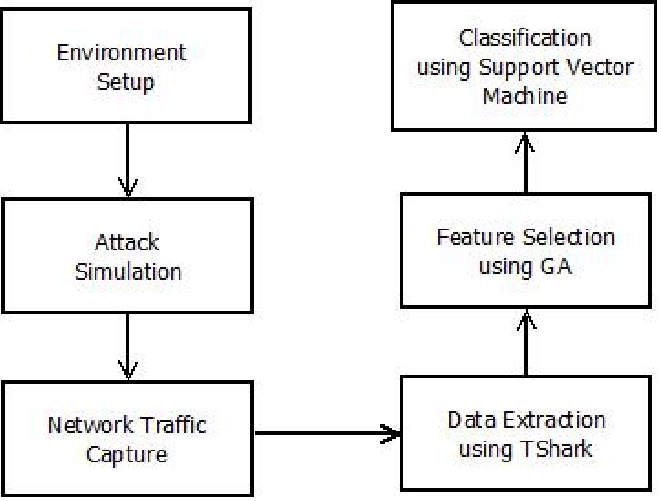
\includegraphics[width=0.80\textwidth]{Images/Block-diagram.png}
    \caption{Block Diagram of the Classification System}
    \label{fig:mlpipeline}
\end{figure}


 

%
%\begin{equation}
%\text{Accuracy} = \frac{TP + TN}{TP + TN + FP + FN}
%\tag{1.1}
%\end{equation}


%\begin{table}[H]
%\centering
%\caption{Sample UCI Heart Disease dataset}
%\begin{tabular}{|c|c|p{1.5cm}|c|p{1.5cm}|c|c|c|p{1.5cm}|}
%\hline
%\textbf{Age} & \textbf{Sex} & \textbf{Chest Pain Type} & \textbf{RestBP} & \textbf{Chole sterol} & \textbf{FastingBS} & \textbf{RestECG} & \textbf{MaxHR} & \textbf{Heart Disease} \\ \hline
%63 & 1 & 3 & 145 & 233 & 1 & 0 & 150 & 1 \\ \hline
%37 & 1 & 2 & 130 & 250 & 0 & 1 & 187 & 0 \\ \hline
%41 & 0 & 1 & 130 & 204 & 0 & 0 & 172 & 0 \\ \hline
%\end{tabular}
%\end{table}


\section{Research Contribution}

{\color{red} \textbf{  Instruction:} “Highlight what is new or unique in the work by mentioning any improvements, comparisons, or simplifications introduced.”}

 \textbf{\color{blue} Example:} Several key contributions were made by this research. A comparison of multiple machine learning algorithms was provided on the same dataset using a minimal set of features, and their relative performance was highlighted.


\section{Financial Planning and Timeline}

\subsection{ Budget Estimation}

{\color{red} \textbf{  Instruction:} Break down the costs of your work if it involves hardware, software, or travel. If costs are not applicable, skip this part or write: “No major cost is involved.”}

 \textbf{\color{blue} Example:} No major costs are involved in this work. All tools and datasets used are open-source and freely available. The development environment runs on a personal laptop.

\subsection{  Gantt Chart }
{\color{red} \textbf{  Instruction:} "Create a visual chart showing your research timeline (tasks vs. weeks/months)".}

 \textbf{\color{blue} Example:} The Fig \ref{fig:planschedule} represents a visual chart of the research timeline for a heart disease prediction project. It outlines the sequence of key tasks, including data collection, data pre-processing, feature selection, model development, training and validation, performance analysis, and deployment preparation. Each task is mapped along a timeline to show the planned duration and order of activities, helping to organize the workflow and track progress throughout the study.


\begin{figure}[ht]
    \centering
    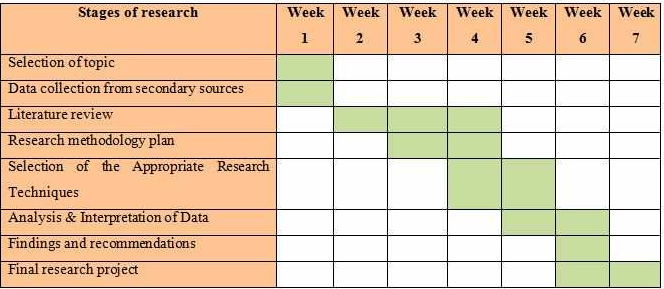
\includegraphics[width=0.90\textwidth]{Images/A planned thesis schedule.png}
    \caption{A planned thesis schedule.}
    \label{fig:planschedule}
\end{figure}



\section{Organization of the Dissertation }

\textbf{\color{blue} Example:}

In this dissertation, the remaining chapters are organized as follows:

Chapter \ref{Literature Review}, \textit{Literature Review}, discusses the existing research related to heart disease prediction. It provides an overview of various machine learning techniques and compares their relative effectiveness in predicting heart diseases.

Chapter \ref{System Architecture}, \textit{Methodology}, describes the dataset employed in this study, the applied feature selection techniques, the process of model development, and the evaluation strategies adopted to assess performance.

Chapter \ref{Results and Discussion}, \textit{Results and Discussion}, presents the experimental outcomes along with graphical representations and offers a comprehensive analysis of the model's predictive performance.

Finally, Chapter \ref{Conclusion}, \textit{Conclusion and Future Work}, summarizes the key findings of this research, outlines its limitations, and provides recommendations for future work and potential improvements.

 \chapter{Literature Review}
\label{Literature Review}





{\color{red} \textbf{Instruction:} A literature review is a comprehensive examination and synthesis of existing scholarly works, including research articles, books, and other relevant sources, about a specific topic or research question. It plays a crucial role in academic writing by establishing the context of the research, identifying gaps and trends in the current knowledge landscape, and providing a theoretical framework for the study. Through a critical evaluation of the literature, it justifies the need for the proposed research, guides methodological choices, and helps avoid redundancy by building upon prior work. The literature review not only assesses the quality and credibility of existing research but also organizes information in a structured manner, categorizing studies based on themes or methodologies. Additionally, it serves as a roadmap for future research by highlighting unanswered questions and areas that warrant further investigation. Overall, a well-conducted literature review contributes to the depth and credibility of academic research, ensuring that the study is situated within the broader scholarly discourse.}











\section{Introduction}

{\color{blue}\textbf{Purpose:}
Set the scope and objectives of the literature review; tell the reader what topics, time span, and types of sources you will cover and why.} \\

{\color{red}\textbf{Writing Instructions (step-by-step):}
\begin{enumerate}
    \item Start with 2–3 short paragraphs that define the scope: subject area, timeframe (e.g., last 10 years), and types of literature (peer-reviewed journals, conference papers, standards, patents).
    
    \item Explicitly state the aims of the review (e.g., ``This review aims to synthesize recent empirical findings on X, evaluate conceptual models Y, and identify gaps relevant to Z'').
    
    \item Describe your search strategy briefly: databases searched (Scopus, IEEE Xplore, Web of Science), keywords, inclusion/exclusion criteria, and date range. Include a short PRISMA-style sentence or a tiny flow line if many sources.
    
    \item Outline how the review is organized (themes, theories, methods, or chronology). Use a short roadmap sentence: ``Section 2.2 reviews theoretical models; 2.3 surveys empirical studies; 2.4 critically compares approaches.''
\end{enumerate}}


\section{Theoretical Background / Existing Models}

{\color{blue}\textbf{Purpose:}
Present the core theories, conceptual models, and formal frameworks that underpin your research — provide the theoretical foundations you will use later.} \\

{\color{red}\textbf{Writing Instructions (step-by-step):}
\begin{enumerate}
    \item Identify and name the principal theories or models relevant to your problem (e.g., queuing theory, socio-technical models, diffusion of innovation, CNN architectures).
    
    \item For each theory/model: give a concise definition, its origin (key citations), formal structure (variables, equations, or components), and why it matters for your work. Use subheadings for each major theory.
    
    \item If applicable, include mathematical formulation or diagrams (labelled figures) to show model components and relationships. Explain notation clearly.
    
    \item Critically evaluate each model: strengths, assumptions, limitations, empirical support. Don't merely summarize — show critical appraisal.
    
    \item Conclude with how these theories inform your conceptual framework or methodological choices (bridge to Chapter 3).
\end{enumerate}}



\section{Related Studies}

{\color{blue}\textbf{Purpose:}
Review empirical and applied research closely related to your research question — demonstrate depth of reading and situate your work within the literature.} \\

{\color{red}\textbf{Writing Instructions (step-by-step):}
\begin{enumerate}
    \item Group studies by theme, method, or application rather than listing paper by paper. Use logical headings (e.g., ``Deep learning approaches,'' ``Rule-based systems,'' ``Field experiments in X'').
    
    \item For each group, synthesize key findings, datasets used, methodologies, evaluation metrics, and reported strengths and weaknesses. Use short comparative tables summarizing essential info (Author | Year | Method | Dataset | Key Result | Limitation).
    
    \item Highlight the most influential/closest works (2–5 anchor papers). Provide slightly deeper critique for these (design choices, parameter settings, reproducibility).
    
    \item Pay attention to methodological details: sample sizes, hyperparameters, baselines, evaluation protocols — note any inconsistencies across studies.
    
    \item Identify patterns — where the literature converges and diverges. Use transitional sentences to lead into gaps.
\end{enumerate}


\begin{itemize}
     \item Review existing literature related to your topic.
     \item Identify key theories, concepts, and research findings.
     \item Discuss the current state of knowledge in the field and gaps that your project/thesis aims to address.
\end{itemize} }


\textbf{ \color{blue} Example:}


\subsection*{Blockchain-Based IoT Access Control System: Towards Security, Lightweight, and Cross-Domain}
Sun et al. propose a blockchain-based access control system tailored for the Internet of Things (IoT) that ensures lightweight performance, cross-domain support, and enhanced security \cite{Sun2021}. The system employs smart contracts and a role-based permission structure to manage access in decentralized IoT environments. It introduces a lightweight consensus mechanism and uses elliptic curve cryptography to reduce overhead.




These limitation are a lack of performance validation under high node scalability. Energy consumption on resource-constrained IoT devices has not been fully evaluated. The paper does not address key revocation in access control.




\begin{longtable}{|p{3cm}|p{7cm}|p{5.0cm}|}
\caption{Literature review summary of blockchain-based certificate verification system} \\
\hline
\textbf{Author(s) (Year)} & \textbf{Contribution} & \textbf{Limitation} \\
\hline
\endfirsthead

\hline
\textbf{Author(s) (Year)} & \textbf{Contribution} & \textbf{Limitation} \\
\hline
\endhead

\hline
\endfoot

Rustemi et al. (2023) \cite{Rustemi2023} & Conducted a \textbf{systematic literature review} on blockchain-based academic certificate verification systems and classified smart contract usage patterns. & \textbf{Limited scope} to certificate verification; did not address \textbf{interoperability or legal compliance}. \\
\hline
KC et al. (2023) \cite{Aloqaily2020} & Developed a system using \textbf{QR code-based issuer validation} and \textbf{blockchain storage} to detect fake physical certificates. & Focused only on \textbf{PDF or printed certificates}; lacks support for \textbf{legacy institutional integration}. \\
\hline
Jadhav et al. (2024) \cite{Ankit2023} & Proposed a \textbf{blockchain-driven smart contract system} for secure issuance and verification of educational certificates. & \textbf{Limited testing} on large-scale deployment and \textbf{no discussion on user privacy or data anonymization}. \\
\hline
Rahman et al. (2023) \cite{Rahman2023} & Proposed an \textbf{AI-integrated blockchain model} for threat detection in educational networks. & \textbf{Too complex for typical academic deployment}; lacks certificate-specific validation logic. \\
\hline

\end{longtable}








\section{Comparative Analysis of Existing Approaches}

{\color{blue}\textbf{Purpose:}
Systematically compare principal approaches, highlighting performance, complexity, scalability, assumptions, and applicability to your problem domain.} \\

{\color{red}\textbf{Writing Instructions (step-by-step):}
\begin{enumerate}
    \item Choose comparison dimensions relevant to your research: accuracy/performance, data requirements, computational cost, generalizability, interpretability, robustness, ethical/privacy concerns.
    
    \item Create a clear, well-labelled comparison table (e.g., TABLE 2.1) with rows as approaches and columns as comparison criteria. Add footnotes for special cases.
    
    \item For each criterion, write a small paragraph interpreting the table: which approaches excel, which fail, and why. Use empirical evidence from literature (cite numbers where possible).
    
    \item Discuss trade-offs explicitly (e.g., approach A gives higher accuracy but requires large labeled data and high compute).
    
    \item Evaluate suitability for your research context and constraints — justify why certain approaches are promising or unsuitable.
\end{enumerate}}


\section{Summary of Research Gaps}

{\color{blue}\textbf{Purpose:}
Synthesize the review to state clearly what is missing in the literature and how your thesis will address these gaps.} \\

{\color{red}\textbf{Writing Instructions (step-by-step):}
\begin{enumerate}
    \item List 3–5 precise, researchable gaps derived from the comparative analysis (e.g., ``Lack of real-world longitudinal evaluation,'' ``Limited explainability in model X,'' ``No integration of privacy preserving methods in Y''). Phrase each gap as a concise sentence.
    
    \item For each gap, explain the consequences of that gap (why it matters) and cite supporting literature.
    
    \item Map gaps to potential research objectives — show how each gap suggests a specific aim or question you will pursue. A small mapping table is excellent: (Gap → Implication → Thesis Objective).
    
    \item End the section with a short paragraph explicitly stating how your study addresses the most critical gap(s) — this bridges to Chapter 3 (Conceptual Framework \& Methodology).
\end{enumerate}}



\textbf{ \color{blue} Example:}Traditional certificate verification methods mainly rely on centralized systems and manual checking, which often leads to document forgery and inefficiency \cite{Aloqaily2020, Rahman2023}. These processes take a lot of time and cause delays in important activities such as job recruitment, student admissions, and other tasks that require quick verification. Centralized databases are also at risk of tampering, forgery, and data manipulation, which reduces transparency and trust \cite{Rahman2023}. In Bangladesh, the verification of myGov.bd certificates are done online, but it still depends on a centralized database without the use of blockchain technology, which limits transparency and resistance to tampering \cite{Rustemi2023} . Globally, there is no universal, secure, and fast method for certificate verification \cite{Ankit2023}. Therefore, there is a clear need for a decentralized, tamper-proof solution to ensure the authenticity, integrity, and quick verification of certificates  \cite{Sun2021}.
 %\chapter{System Architecture}
\chapter{Proposed Methodology}
\label{System Architecture}



\section{Introduction}

{\color{blue}\textbf{Purpose:}
Provide an overview of what the chapter covers — the conceptual structure of your study, theoretical foundations, and the system or model architecture.} \\

{\color{red}\textbf{Writing Instructions:}
\begin{enumerate}
    \item Start with a short paragraph linking from Chapter 2: ``Building on the insights gained from the literature review, this chapter develops the conceptual and system framework underlying the study.''
    
    \item Explain the structure of the chapter: what frameworks, models, or methodologies will be presented.
    
    \item Mention the logical flow — from theoretical conception to system design or implementation approach.
\end{enumerate}}




\section{Conceptual Framework}

{\color{blue}\textbf{Purpose:}
Define and explain the conceptual or theoretical model that guides your study. This framework demonstrates how variables, processes, or modules interact to solve your research problem.} \\

{\color{red}\textbf{Writing Instructions:}
\begin{enumerate}
    \item Begin with a definition of what your conceptual framework represents (e.g., theoretical model, workflow, system process, or hypothesis network).
    
    \item Include a diagram (Figure 3.1) that visually represents the framework.
    
    \item Use labeled boxes and arrows to show relationships or data flow.
    
    \item Follow IEEE figure formatting (caption below, sentence case).
    
    \item Describe each component of the diagram in clear, numbered paragraphs.
    
    \item Explain the purpose, relationship, and expected function of each part.
    
    \item Justify your framework design based on literature (refer back to Chapter 2).
    
    \item End with a summary linking how this conceptual model will guide system design or methodology in later sections.
\end{enumerate}}

\section{System Architecture}

{\color{blue}\textbf{Purpose:}
Translate the conceptual framework into a technical or methodological architecture — the practical structure of your research system, model, or experimental setup.} \\

{\color{red}\textbf{Writing Instructions:}
\begin{enumerate}
    \item Begin with a paragraph summarizing the general system design approach — what kind of architecture is used (layered, modular, client–server, pipeline, etc.).
    
    \item Present a system architecture diagram (Figure 3.2).
    
    \item Describe each system component (software modules, data sources, processing units).
    
    \item Explain how these components interact to fulfill research objectives.
    
    \item Include methodology flow if this involves experimental research (input → process → output).
    
    \item Reference tools and techniques briefly (details will appear in implementation or Chapter 4).
\end{enumerate}


\textbf{Instruction:} Methodology refers to the systematic and structured approach used in a research study to gather, analyze, and interpret data. It outlines the specific procedures, techniques, and tools employed to address the research questions or objectives. A well-defined methodology provides a clear roadmap for the research process, ensuring the reliability and validity of the study. This section typically includes details on the research design, sampling methods, data collection techniques, and data analysis procedures. The methodology allows other researchers to replicate the study and assess its rigor. It plays a critical role in establishing the credibility of research findings and is essential for drawing meaningful conclusions from the collected data. }



\begin{figure}[ht]
    \centering
    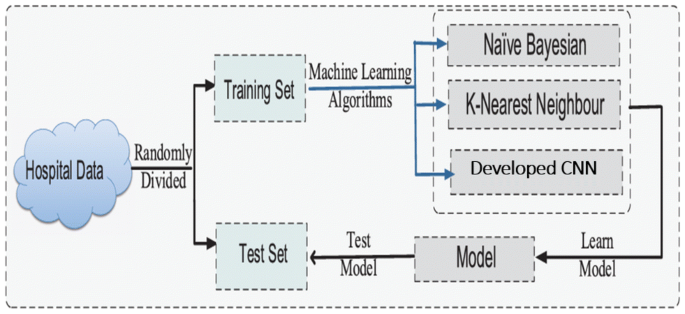
\includegraphics[width=0.90\textwidth]{Images/ML pipeline for detection task on medical imaging data.png}
    \caption{A ML pipeline for detection task on medical imaging data.}
    \label{fig:mlpipeline1}
\end{figure}


\subsection{Algorithms and Model Explanation}

{\color{blue}\textbf{Purpose:}
Describe the computational or logical methods used in your research — algorithms, formulas, or models that underpin your system.} \\

{\color{red}\textbf{Writing Instructions:}
\begin{enumerate}
    \item Write algorithm steps in numbered pseudocode format (use Algorithm environment in LaTeX).
    
    \item Include any mathematical equations (clearly numbered as Eq. 3.1, Eq. 3.2).
    
    \item Explain the logic of your model — how inputs are transformed into outputs.
    
    \item Describe parameter settings, training process (if ML model), or logical flow.
    
    \item Provide a complexity or performance analysis if applicable (Big-O, time, memory, etc.).
\end{enumerate}}


\subsection{Data Flow Diagram (if applicable)}

{\color{blue}\textbf{Purpose:}
Illustrate how data moves within the system — from input to storage, processing, and output.}

{\color{red}\textbf{Writing Instructions:}
\begin{enumerate}
    \item Use standard DFD notations (process, data store, data flow, external entity).
    
    \item Present Level-0 (context) and Level-1 diagrams if your system is complex.
    
    \item Label all entities and flows clearly.
    
    \item Describe each process in 1–2 sentences under the figure.
    
    \item Ensure the diagram corresponds exactly to the modules described earlier.
\end{enumerate}


\begin{itemize}
    \item Describe the research design, methods, and procedures used in your project/thesis.
    \item Explain the data collection/requirement identification and analysis techniques.
    \item Discuss any ethical considerations and limitations of your study.
\end{itemize}}



\section{Data Collection Process and Analysis}

{\color{blue}\textbf{Purpose:}
Explain how data is collected, processed, and analyzed in your study — bridging design with analytical methodology.} \\

{\color{red}\textbf{Writing Instructions:}
\begin{enumerate}
    \item Start by explaining your data flow process (collection → preprocessing → analysis).
    
    \item Justify the choice of data source — show reliability and relevance.
    
    \item Explain data preparation steps (cleaning, normalization, feature extraction).
    
    \item Describe analysis techniques — statistical, computational, or experimental.
    
    \item Present sample formats, variables, or data schema diagrams if applicable.
    
    \item Mention tools or software used for analysis (e.g., Python, MATLAB, R).
\end{enumerate}


Data presentation and analysis constitute a pivotal phase in the research process, where collected information is organized, interpreted, and communicated effectively. In this stage, raw data are transformed into meaningful insights through various statistical or qualitative methods, depending on the research design. Data presentation involves visually representing the findings using tables, charts, graphs, or other visual aids to enhance clarity and comprehension. Analysis, on the other hand, encompasses the systematic examination of the data to uncover patterns, relationships, and trends. This process not only validates the research outcomes but also enables researchers to draw meaningful conclusions and make informed interpretations. Effectively presenting and analyzing data is essential for conveying the significance of the research findings to both academic and non-academic audiences. 

\begin{itemize}
    \item Present the data collected during your project.
    \item Use tables, graphs, charts, or other visuals to enhance clarity.
    \item Analyze the data and draw conclusions based on your findings.
\end{itemize} }




\subsection{ Data Collection Methods}

{\color{blue}\textbf{Purpose:}
Document the techniques used to gather information, datasets, or experimental measurements.} \\

{\color{red}\textbf{Writing Instructions:}
\begin{enumerate}
    \item State clearly what type of data (primary, secondary, simulated, experimental).
    
    \item Describe the instruments, sources, or platforms used (surveys, sensors, APIs, etc.).
    
    \item Explain data validation (quality control, filtering, calibration).
    
    \item If using human participants, note ethical approval and consent.
\end{enumerate}}

\subsection{Data Analysis Techniques}

{\color{blue}\textbf{Purpose:}
Explain how raw data is transformed into meaningful information.}

{\color{red}\textbf{Writing Instructions:}
\begin{enumerate}
    \item Describe statistical, computational, or analytical techniques used (e.g., regression, clustering, hypothesis testing, evaluation metrics).
    
    \item Justify why each method was chosen.
    
    \item Present formulae, tools, or frameworks used.
    
    \item Discuss limitations or assumptions (normality, independence, etc.).
\end{enumerate}}

\section{Engineering and Societal Considerations}
{\color{blue}\textbf{Purpose:}
Demonstrate professional responsibility — that your design or system adheres to ethical, environmental, and social standards.} \\

{\color{red}\textbf{Writing Instructions:}
\begin{enumerate}
    \item Introduce the idea that technical innovation must align with engineering ethics and sustainability.
    
    \item Divide into three key subsections: societal impact, environmental considerations, and ethical responsibility.
    
    \item Use real examples (e.g., carbon footprint, accessibility, data privacy).
    
    \item Link your considerations to relevant global frameworks (IEEE Code of Ethics, SDGs, GDPR).
\end{enumerate}

Engineering considerations encompass a set of crucial factors that engineers must weigh during the design, development, and implementation of projects.}

\subsection{Societal Impacts of Engineering Solutions}

{\color{blue}\textbf{Purpose:}
Evaluate how your system affects people, communities, or industries.} \\

{\color{red}\textbf{Writing Instructions:}
\begin{enumerate}
    \item Discuss both positive outcomes (efficiency, inclusion) and potential negative effects (job displacement, privacy risks).
    
    \item Relate to real-world case studies or applications.
    
    \item Emphasize alignment with human-centered design principles.
\end{enumerate}

The relationship between the engineer and society involves recognizing the societal impacts of engineering solutions, including considerations for safety, accessibility, and the overall well-being of communities. Engineers are increasingly mindful of their role in promoting social responsibility and addressing diverse needs.}

\subsection{Environment and Sustainability Considerations}

{\color{blue}\textbf{Purpose:}
Assess your system’s environmental footprint and contribution to sustainability.} \\

{\color{red}\textbf{Writing Instructions:}
\begin{enumerate}
    \item Discuss energy efficiency, hardware usage, or green data practices.
    
    \item Show how your work supports one or more UN Sustainable Development Goals (SDGs).
    
    \item Mention design decisions that reduce resource use or waste.
\end{enumerate}

Environment and sustainability considerations involve assessing and mitigating the environmental impact of engineering projects. This includes minimizing resource depletion, reducing pollution, and promoting sustainable practices to ensure long-term ecological balance. Sustainable engineering aims to create solutions that meet present needs without compromising the ability of future generations to meet their own needs.}

\subsection{Ethical and Professional Responsibility}

{\color{blue}\textbf{Purpose:}
Show compliance with ethical standards and academic integrity.} \\

{\color{red}\textbf{Writing Instructions:}
\begin{enumerate}
    \item Reference professional codes (IEEE, ACM, ISO, Belmont Report).
    
    \item Mention data privacy, informed consent, plagiarism avoidance, and responsible AI (if relevant).
    
    \item Include institutional approval if human data are used.
\end{enumerate}
Ethics in engineering emphasizes the moral and professional responsibilities of engineers. Ethical considerations involve ensuring the safety, honesty, and integrity of engineering practices. Engineers are expected to prioritize the well-being of individuals and communities, uphold transparency, and adhere to ethical codes in their decision-making processes.}

 \chapter{Results and Discussion}
\label{Results and Discussion}

{\color{blue}\textbf{Purpose:}
Briefly introduce what this chapter covers — summarize how results were obtained and how they will be analyzed.} \\

{\color{red}\textbf{Writing Instructions:}
\begin{enumerate}
    \item Begin by linking this chapter to your methodology:  
    ``This chapter presents the experimental results and analytical findings obtained from implementing the proposed system described in Chapter 3.''
    
    \item Outline the organization of this chapter — e.g., quantitative analysis, qualitative evaluation, comparison, discussion.
    
    \item Mention the goals of your analysis — what questions or hypotheses the results will address.
\end{enumerate}


Results and discussions represent critical sections of a research report where the findings of a study are presented and analyzed. The results section provides a straightforward presentation of the collected data, often through tables, figures, or statistical summaries. This section is focused on conveying the outcomes of experiments, surveys, or analyses, without interpretation or discussion.

Following the results, the discussion section delves into the interpretation and analysis of the presented data. Researchers provide context for their findings by relating them to the research question, hypothesis, or existing literature. It involves a critical examination of the significance of the results, identification of patterns or trends, and exploration of potential implications for the field of study.

In the discussion section, researchers may also address unexpected results, limitations of the study, and avenues for future research. The goal is to provide a comprehensive understanding of the research outcomes and their broader implications, fostering a deeper comprehension of the study within the academic community. The results and discussion sections collectively contribute to the overall coherence and impact of the research report.}

\section{Introduction}

{\color{blue}\textbf{Purpose:}
Mention your simulation environment, hardware/software systems, packages, libraries, etc. Present the raw outcomes of your experiments, models, or system tests clearly, systematically, and objectively.} \\

{\color{red}\textbf{Writing Instructions:}
\begin{enumerate}
    \item Use subheadings or tables/figures to organize your findings logically.
    
    \item Present quantitative outputs (numerical, graphical) and qualitative observations (patterns, behaviors).
    
    \item Use IEEE-compliant figure and table captions:
    \begin{itemize}
        \item Table captions above tables (e.g., TABLE I. Performance Metrics)
        \item Figure captions below figures (e.g., Fig. 4.1. Accuracy vs. Epochs Curve).
    \end{itemize}
    
    \item Avoid interpretation here — simply describe what you observed.
    
    \item Use visuals effectively: bar charts, line plots, confusion matrices, etc.
\end{enumerate}}


\section{Quantitative Results}

{\color{blue}\textbf{Purpose:}
Present measurable numerical data from experiments, simulations, or model evaluations.} \\

{\color{red}\textbf{Writing Instructions:}
\begin{enumerate}
    \item Introduce the metrics used (e.g., Accuracy, Precision, Recall, F1-score, RMSE, Throughput).
    
    \item Present results systematically — one metric or scenario per subsection.
    
    \item Use tables (IEEE-style) for numerical summaries and graphs for trends.
    
    \item Discuss the significance of results — e.g., ``The 95\% confidence interval indicates robust model performance.''
    
    \item Use comparison plots (e.g., proposed model vs. baseline).
\end{enumerate}}

\subsection{Performance Metrics}

{\color{blue}\textbf{Purpose:}
Define and explain how each metric is computed and why it’s relevant.} \\

{\color{red}\textbf{Writing Instructions:}
\begin{enumerate}
    \item Define every metric mathematically if possible (Eq. 4.1, Eq. 4.2).
    
    \item Discuss how these metrics align with your research objectives.
    
    \item Compare your system’s metrics with existing studies or baselines.
\end{enumerate}}

\subsection{Result Tables and Graphical Representations}

{\color{blue}\textbf{Purpose:}
Visually communicate findings for easy understanding.} \\

{\color{red}\textbf{Writing Instructions:}
\begin{enumerate}
    \item Use concise, properly labeled tables and charts.
    
    \item Avoid redundancy — do not repeat the same data in both table and graph.
    
    \item Maintain consistent color coding and axis scales.
    
    \item Ensure captions are complete and follow IEEE format.
\end{enumerate}}


\subsection{Statistical Analysis (if applicable)}

{\color{blue}\textbf{Purpose:}
Demonstrate the reliability and validity of your data through statistical tests.} \\

{\color{red}\textbf{Writing Instructions:}
\begin{enumerate}
    \item Describe statistical tests used (t-test, ANOVA, correlation, regression).
    
    \item Include p-values or confidence levels to show result significance.
    
    \item Interpret what the statistical outcomes mean for your hypothesis.
\end{enumerate}}



\section{Qualitative Results}

{\color{blue}\textbf{Purpose:}
Show the non-numerical outcomes — user experience, case studies, or observed behavioral patterns.} \\

{\color{red}\textbf{Writing Instructions:}
\begin{enumerate}
    \item Introduce qualitative evaluation goals — usability, efficiency, satisfaction, etc.
    
    \item Present user or case study results (e.g., interview feedback, expert reviews).
    
    \item Summarize findings using short quotes or thematic categories.
    
    \item Visualize using screenshots, workflow images, or comparative case summaries.
\end{enumerate}}


\subsection{Visualization of Results}

{\color{blue}\textbf{Purpose:}
Show how your results manifest visually or through system interfaces.} \\

{\color{red}\textbf{Writing Instructions:}
\begin{enumerate}
    \item Include screenshots, model outputs, dashboards, or visual patterns.
    
    \item Explain each visualization in context — what it shows and why it matters.
    
    \item Use clear figure numbering (e.g., Fig. 4.5. Visualization of Model Output).
\end{enumerate}}


\subsection{User Evaluation / Case Studies (if applicable)}

{\color{blue}\textbf{Purpose:}
Validate your system’s effectiveness from a user or real-world perspective.} \\

{\color{red}\textbf{Writing Instructions:}
\begin{enumerate}
    \item Describe test participants or case study context.
    
    \item Explain evaluation process (surveys, testing, observation).
    
    \item Summarize findings objectively — use statistics or summary tables if available.
    
    \item Mention feedback insights and improvement opportunities.
\end{enumerate}}



\section{Comparative Analysis}

{\color{blue}\textbf{Purpose:}
Compare your proposed system or model against existing benchmarks or literature results.} \\

{\color{red}\textbf{Writing Instructions:}
\begin{enumerate}
    \item Select 3–5 prior studies or baseline systems for comparison.
    
    \item Present a comparison table summarizing metrics (accuracy, cost, time, etc.).
    
    \item Discuss relative strengths and weaknesses.
    
    \item Use graphs for visual comparison (e.g., performance bar charts).
\end{enumerate}}



\subsection{Benchmark Comparison}

{\color{blue}\textbf{Purpose:}
Quantitatively show superiority or improvement over established baselines.} \\

{\color{red}\textbf{Writing Instructions:}
\begin{enumerate}
    \item Define benchmark datasets or models.
    
    \item Present results in tabular form side-by-side.
    
    \item Highlight improvements in bold or color-coded text.
\end{enumerate}}

\subsection{Correlation with Literature Review}

{\color{blue}\textbf{Purpose:}
Position your findings within the context of existing knowledge.} \\

{\color{red}\textbf{Writing Instructions:}
\begin{enumerate}
    \item Compare your outcomes with prior studies.
    
    \item Discuss agreement or contradiction with previous research.
    
    \item Mention possible reasons for differences (data size, methods, tools).
\end{enumerate}}

\subsection{Discussion of Improvements}

{\color{blue}\textbf{Purpose:}
Explain why your system outperforms others.} \\

{\color{red}\textbf{Writing Instructions:}
\begin{enumerate}
    \item Link design decisions or innovations to better results.
    
    \item Support claims with evidence (graphs, equations, user tests).
    
    \item Address any limitations or trade-offs.
\end{enumerate}}


\section{Discussion of Findings}

{\color{blue}\textbf{Purpose:}
Synthesize all results and connect them back to research goals and theory.} \\

{\color{red}\textbf{Writing Instructions:}
\begin{enumerate}
    \item Restate research objectives briefly.
    
    \item Summarize whether results meet those objectives.
    
    \item Correlate findings with literature (Chapter 2).
    
    \item Highlight new insights or patterns.
    
    \item Identify implications for future research or industry application.
\end{enumerate}}





 \chapter{Conclusion}
\label{Conclusion}



\section{Summary of the Study}

{\color{blue}\textbf{Purpose:}
Provide a concise recap of your entire research — what was done, how it was done, and what was achieved.} \\

{\color{red}\textbf{Writing Instructions:}
\begin{enumerate}
    \item Begin by restating your research topic and purpose in one sentence.\\
    ``This study aimed to develop and evaluate a system for…''
    
    \item Summarize each chapter briefly (2–3 lines per chapter):
    \begin{itemize}
        \item Chapter 1: Problem and objectives
        \item Chapter 2: Literature findings
        \item Chapter 3: Methodology or system framework
        \item Chapter 4: Key results and discussion
    \end{itemize}
    
    \item End by stating the core outcomes and what new insights the study has produced.
    
    \item Keep it concise — around 300–400 words.
\end{enumerate}}


\section{Key Findings and Contributions}

{\color{blue}\textbf{Purpose:}
Highlight the original achievements and scientific or practical contributions of your work.} \\

{\color{red}\textbf{Writing Instructions:}
\begin{enumerate}
    \item List your main findings clearly and sequentially.\\
    ``The model achieved a 92\% accuracy in…''\\
    ``User feedback indicated a 40\% improvement in…''
    
    \item Then, explain the contributions of your research:
    \begin{itemize}
        \item Theoretical Contribution: New framework, concept, or algorithm.
        \item Practical Contribution: System, prototype, or application.
        \item Methodological Contribution: New approach, metric, or analysis method.
    \end{itemize}
    
    \item Compare with prior work to show novelty.
\end{enumerate}

\begin{itemize}
    \item Summarize the key points of your project/thesis.
    \item Reinforce the significance of your findings.
    \item Suggest areas for further research or improvement.
\end{itemize}}

\section{Limitations}

{\color{blue}\textbf{Purpose:}
Acknowledge constraints that affected your study’s design, execution, or outcomes.} \\

{\color{red}\textbf{Writing Instructions:}
\begin{enumerate}
    \item Identify limitations objectively — data size, time, hardware, funding, or scope.
    
    \item Discuss how these limitations might have influenced your findings.
    
    \item Emphasize how future work can address them.
    
    \item Avoid defensive or apologetic language — present them as opportunities for growth.
\end{enumerate}}


\section{Future Works}

{\color{blue}\textbf{Purpose:}
Propose logical and realistic directions for extending your research.} \\

{\color{red}\textbf{Writing Instructions:}
\begin{enumerate}
    \item Present 3–5 actionable recommendations for future studies.
    \begin{itemize}
        \item Improving system scalability or accuracy.
        \item Testing on different datasets or environments.
        \item Integrating emerging technologies (e.g., blockchain, AI, IoT).
        \item Conducting long-term evaluation or field deployment.
    \end{itemize}
    
    \item Prioritize ideas that build directly on your findings.
    
    \item Use future-oriented language (``Future research may explore…'').
\end{enumerate}}


\section{Recommendations}

{\color{blue}\textbf{Purpose:}
Provide practical or policy-level suggestions based on your findings — often aimed at industry, academia, or policymakers.} \\

{\color{red}\textbf{Writing Instructions:}
\begin{enumerate}
    \item Frame recommendations from evidence — do not generalize.
    
    \item Divide into categories if relevant:
    \begin{itemize}
        \item Technical Recommendations — ``Adopt modular architecture for scalability.''
        \item Policy Recommendations — ``Encourage data transparency and open-source collaboration.''
        \item Educational Recommendations — ``Integrate research insights into academic curricula.''
    \end{itemize}
    
    \item Support each recommendation with a rationale from your results.
\end{enumerate}}


\section{Concluding Remarks}

{\color{blue}\textbf{Purpose:}
End the thesis with a final reflective statement — emphasizing the broader significance and potential of your research.} \\

{\color{red}\textbf{Writing Instructions:}
\begin{enumerate}
    \item Write 1–2 strong closing paragraphs:
    \begin{itemize}
        \item Reflect on the impact of your research (academic, social, industrial).
        \item Emphasize how your study contributes to solving a real-world problem.
        \item Reaffirm your commitment to continuous exploration.
    \end{itemize}
    
    \item Avoid repetition; aim for inspiration and closure.
    
    \item End with a thought-provoking line such as:\\
    ``While this study concludes here, it marks the beginning of a broader exploration into intelligent and ethical computing for society.''
\end{enumerate}


\begin{itemize}
    \item Provide practical recommendations based on your thesis/project's findings.
    \item Discuss potential actions or strategies that could address the identified problem.
\end{itemize}}

  \input{./Setup/rear}  %include Reference Section
 \include{./Chapters/chapter6} %include Appendices Section
 \include{./Chapters/chapter7} % This chapter like usermanual


  \coverpage{\numberOfAuthors}
%-----------------------------------------------------------

\end{document}